\documentclass{zjureport}
% =============================================
% Part 1 Edit the info
% =============================================
\usepackage{indentfirst}
\usepackage{graphicx}
\usepackage{caption}
\newcommand{\major}{计算机应用技术,精密仪器及机械}
\newcommand{\name}{杜沈达,王晨}
\newcommand{\stuid}{SA18168163,SA18168095}
\newcommand{\newdate}{2018-10-24}
\newcommand{\loc}{物理楼}

\newcommand{\course}{光信息科学与技术实验}
\newcommand{\tutor}{光信息科学实验室}
\newcommand{\grades}{}
\newcommand{\newtitle}{实验1-实验5}
\newcommand{\exptype}{验证计算实验}
%\newcommand{\group}{王晨}

% =============================================
% Part 1 Main document
% =============================================
\begin{document}
\thispagestyle{empty}
\begin{figure}[h]
  \begin{minipage}{0.6\linewidth}
    \centerline{\includegraphics[width=\linewidth]{head.jpg}}
  \end{minipage}
  \hfill
  \begin{minipage}{.4\linewidth}
    \raggedleft
    \begin{tabular*}{.8\linewidth}{ll}
      专业: & \underline\major   \\
      姓名: & \underline\name    \\
      学号: & \underline\stuid   \\
      日期: & \underline\newdate \\
      地点: & \underline\loc
    \end{tabular*}
  \end{minipage}
\end{figure}

\begin{table}[!htbp]
  \centering
  \begin{tabular*}{\linewidth}{llllll}
    课程名称: & \underline\course   & 实验名称: & \underline\newtitle   & 成绩:       &  \underline\grades \\
   % 实验名称: & \underline\newtitle & 实验类型: & \underline\exptype & 
    %同组学生姓名:& \underline\group
  \end{tabular*}
\end{table}

% =============================================
% Part 2 Main document
% =============================================

\section{半导体激光器的光学特性测试}
\subsection{实验数据处理}
\begin{clause}
	\item 实验原始数据如下\\
	\begin{center}
	\begin{tabular}{|c|c|}
		\multicolumn{2}{c}{表1.1 半导体激光器的偏振度的测量}\\\hline
		$P_{max}$(mW)&	$P_{min}$(mW)\\\hline
		1.8	&		0.038\\\hline
		计算公式&$p=\frac{P_{max}-P_{min}}{P_{max}+P_{min}}$\\\hline	
		偏振度p	&0.958650707\\\hline	
	\end{tabular}
	\end{center}
	\begin{center}
		\begin{tabular}{|c|c|c|c|c|c|c|c|c|c|c|c|}
			\multicolumn{11}{c}{表1.2 电流功率数据}\\\hline
			组数&1&2&3&4&5&6&7&8&9&10&11\\\hline
			$I$(mA)&0&10&20&30&40&50&60&70&75&80&81\\\hline		
			$P$(mW)&0.0099&	0.0109&0.0142&	0.0194&	0.0245&	0.0307&	0.0392&	0.055&	0.07&	0.1035&0.1154\\\hline
			组数&11&12&13&14&15&16&17&18&19&20&21\\\hline
			$I$(mA)&82&83&84&85&86&88&90&92&94&96&98\\\hline		
			$P$(mW)&0.1323&0.1589&0.2084&0.3202&0.662&2.272&3.942&5.69&	7.33&9.04&10.77\\\hline
		\end{tabular}
	\end{center}
	\begin{center}
		\begin{tabular}{|c|c|c|c|c|c|c|c|c|c|c|}
			\multicolumn{11}{c}{表1.3 半导体激光器的发散角的测定}\\\hline
				组数&1&2&3&4&5&6&7&8&9&10\\\hline
				$\phi(^{\circ})$&0&10&20&30&34&36&38&40&42&44\\\hline
				$P$(mW)&9.2&9.2&9.2&28.5&53.9&73&94.2&114.3&125.1&124.3\\\hline
				组数&11&12&13&14&15&16&17&18&19&20\\\hline
				$\phi(^{\circ})$&46&48&50&52&56&60&70&80&90&100 \\\hline
				$P$(mW)&110.8&92.8&67.1&49.2&22.7&14.1&10.4&9.5&9.5&9.5 \\\hline
		\end{tabular}
	\end{center}
	\item 数据计算处理过程:
	
		\begin{itemize}
			\item[a.] 对于半导体激光器的P-I曲线,根据在实验室测得的数据,先画数据的散点图,再将其连成一条线,使用MATLAB绘制其P-I曲线。
			\item[b.] 对于半导体激光发散角的确定,根据数据画出其散点图,然后画出其曲线图,但是可以看到,这个曲线理论上应该是正态分布曲线,但是因为测量的数据不够多有折点出现,不够光滑,所以使用了MATLAB光滑曲线命令spcrv使得曲线变得光滑,等到光滑处理之后,可以看到,曲线的形式与正态分布曲线十分相似。画出曲线之后,应该找到曲线极值一半的位置画一条水平线来得到横坐标$\phi_{1}$和$\phi_{2}$的值,它们之间的差值$\Delta\phi$就是所求的发散角。\\
			计算过程中,首先使用MATLAB的findpeak命令找到极值所在的位置(点(35,124)),记下其极值的大小,再将极值的一半保留下来,画出y=极值的一半水平线(也就是图中的y=62线),再使得曲线的纵坐标值y是该值,求出横坐标,当然,在此时是有精度的,因为spcurv之后的曲线的构成实际上也是不断插值取数据点的过程,但是在做插值的时候发现,纵坐标和横坐标的范围变化比例大概在100:1,所以控制纵坐标的误差为$\pm1$即可保证横坐标的误差在$\pm0.01$之间。经过计算得到对应到曲线上面找到此时y所对应的$\phi_{1}$和$\phi_{2}$分别为$35^{\circ}$和$51^{\circ}$(此时四舍五入了,实际计算的时候取得是精确值),相减得到差值$\Delta\phi=15.5371^{\circ}$。
		\end{itemize}
	
		
	
	\item 处理结果如下图所示
	\begin{center}
				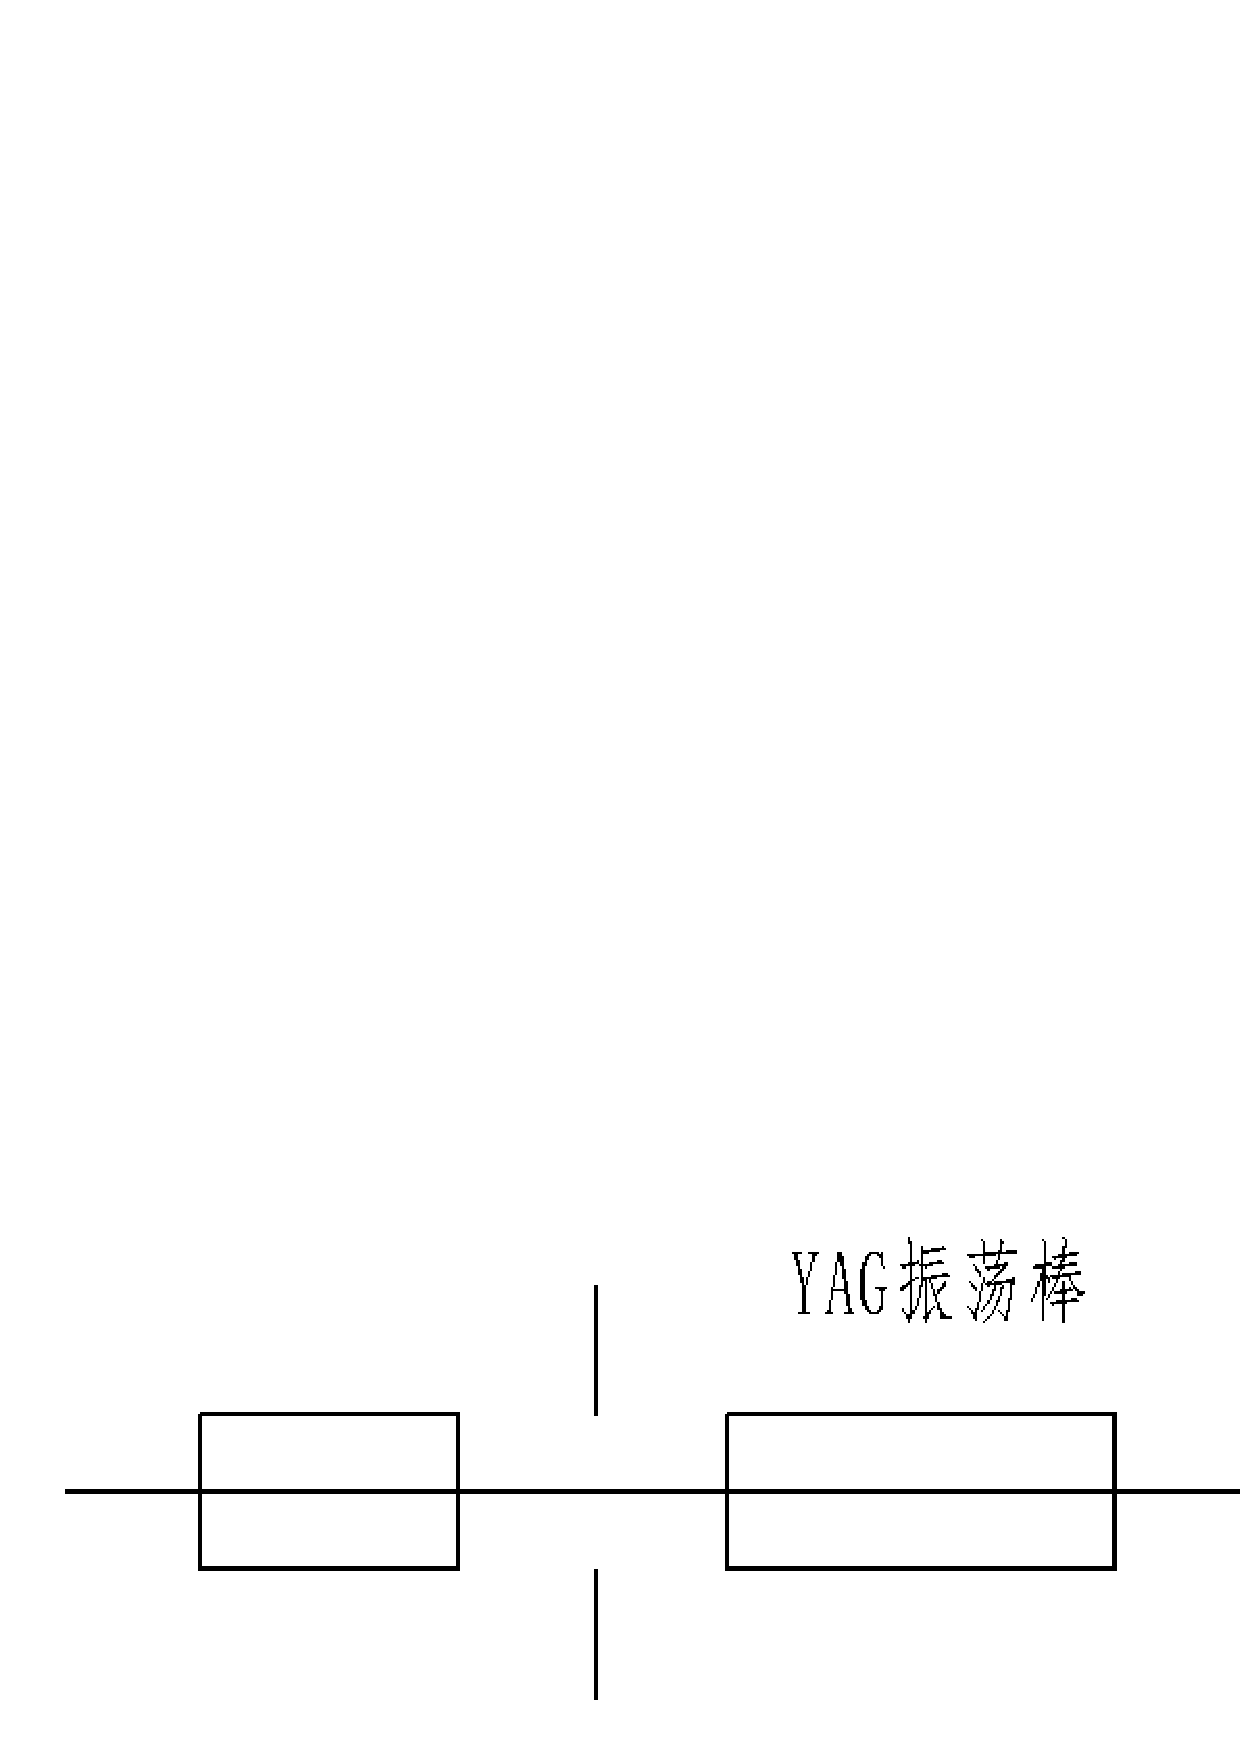
\includegraphics[width=0.6\linewidth]{1.jpg}	
			%	\includegraphics[width=0.6\linewidth]{11.jpg}
	\end{center}
	\item MATLAB代码如下
	\begin{lstlisting}[language=MATLAB]

%半导体激光器的光学特性测试
clear;clc;
data_PI = xlsread('C:\Users\shenda\Desktop\实验.xlsx','sheet1','A3:B24');
figure(1)
subplot(1,2,1);
scatter(data_PI(:,1),data_PI(:,2));
xlabel('电流I(mA)');
ylabel('功率P(mW)');
title('半导体激光器的P-I曲线测量点');
set(gca,'FontSize',10,'Fontname','New Times Roman');
subplot(1,2,2)
plot(data_PI(:,1),data_PI(:,2),'linewidth',2);
xlabel('电流I(mA)');
ylabel('功率P(mW)');
title('半导体激光器的P-I曲线');
set(gca,'FontSize',10,'Fontname','New Times Roman');
box off
print -djpeg -r600 半导体激光器P-I曲线
data_Pphi = xlsread('C:\Users\shenda\Desktop\实验.xlsx','sheet1','G3:H22');
figure(2)
subplot(3,1,1);
scatter(data_Pphi(:,1),data_Pphi(:,2));
xlabel('发散角\phi(°)');
ylabel('功率P(mW)');
title('半导体激光器发散角散点图');
set(gca,'FontSize',10,'Fontname','New Times Roman');
subplot(3,1,2);
plot(data_Pphi(:,1),data_Pphi(:,2),'linewidth',2);
xlabel('发散角\phi(°)');
ylabel('功率P(mW)');
title('半导体激光器发散角测定曲线');
set(gca,'FontSize',10,'Fontname','New Times Roman');
[peaks,locs]=findpeaks(data_Pphi(:,2),'minpeakheight',-5,'minpeakdistance',1)
box off
subplot(3,1,3)
values = spcrv(data_Pphi');
plot(values(1,:),values(2,:), 'b','linewidth',2);
xlabel('发散角\phi(°)');
ylabel('功率P(mW)');
title('光滑处理后的半导体激光器发散角测定曲线');
set(gca,'FontSize',10,'Fontname','New Times Roman');
[peak,loc] = findpeaks(values(2,:),'minpeakheight',100,'minpeakdistance',50);
hold on
plot(values(1,loc),peak,'ro');
str = (['(',num2str(round(values(loc))),',',num2str(round(peak)),')']);
text(values(1,loc)+1,peak+2,str);
half = peak/2;
hold on
x=30:1:60;
y=half+0*x;
plot(x,y);
text(60,half,'极值的一半位置');
min=half-values(2,1);
for i=1:1:139
	if(values(2,i)<half)
		if min>half-values(2,i)
			min = half - values(2,i);
		end
		else
		break;
	end
end
for j=1:139
	if(values(2,139-j)>half)
	break
	end
end
halfx1=(values(1,i)+values(1,i+1))/2;
halfx2=(values(1,139-j)+values(1,139-j+1))/2;
delta_phi = halfx2-halfx1;
plot(halfx1,half,'r*',halfx2,half,'r*');
str1=(['(',num2str(round(halfx1)),',',num2str(round(half)),')']);
str2=(['(',num2str(round(halfx2)),',',num2str(round(half)),')']);
text(halfx1+1,half+6,str1);
text(halfx2+1,half+6,str2);
disp('Δφ=');
disp(delta_phi);
box off
text(35,half-10,['\Delta\phi=',num2str(delta_phi),'°']);
set(gcf, 'PaperPositionMode', 'manual');
set(gcf, 'PaperUnits', 'points');
set(gcf, 'PaperPosition', [0 0 1200 1080]);
print -djpeg -r600 半导体激光器发散角测定曲线
	\end{lstlisting}
\end{clause}
 \subsection{思考题}
 \begin{clause}
 	\item 为什么半导体发光二极管的特征发射线宽为几百埃,而半导体激光器的线宽近似于1埃?\\
 	\item 半导体激光器输出光的准直性如何?(给出典型的发射角)怎么样得到较大的准直性?
 	\item 如果GaAs介质折射率n=3.6,试求GaAs半导体激光器谐振腔端面的反射率R?
 	\item 如果半导体激光器结区的厚度为$1\mu m$,按照图5-10光路所给的数据,由半导体激光器光源限度引起剪切条纹的第一次消失点离双频光栅的轴向距离是多少?
 	~\\
 	~\\
 	~\\
 	~\\
 	~\\
 	~\\
 	~\\
 	~\\
 	~\\
 	~\\
 	~\\
 	~\\
 	~\\
 	~\\
 	~\\
 \end{clause}
 \subsection{做实验和处理数据过程中的问题}
	~\\
~\\
~\\
~\\
~\\
~\\
~\\
~\\
~\\
~\\
~\\
~\\
~\\
~\\
~\\
  \subsection{做完实验的感悟}
 	~\\
 	~\\
 	~\\
 	~\\
 	~\\
 	~\\
 	~\\
 	~\\
 	~\\
 	~\\
 	~\\
 	~\\
 	~\\
 	~\\
 	~\\
\subsection{参考资料}
 \begin{clause}
 \item T.Tamir:“Integrated Optics:Thery and... Techonology",Springerverlag.Tokyo,1984
 \item 明海,张国平,谢建平;“光电子技术",中国科学技术大学出版社,合肥,1998
 \item 明海,李明,陈农,谢建平;“半导体光剪切干涉仪",《中国激光》,Vol,16,No.7(1989)
 \end{clause}
 
\section{光纤光栅温度传感特性测试}

  \subsection{处理结果}

   \begin{clause}
   	\item 实验原始数据如下
   	\begin{center}
   		\begin{tabular}{|c|c|c|c|c|c|c|c|c|}
   			\multicolumn{9}{c}{表2.1 温度与波长数据}\\\hline
   			$\lambda$(nm)&1540.164&	1540.178&1540.211&	1540.259&	1540.293&	1540.602&1540.532&1540.717\\\hline
   			$T(\textcelsius)$&24&27&31&35&38&69&61&79\\\hline
   		\end{tabular}
   	\end{center}
   	\item 数据计算处理过程
   		根据理论,实验测得的温度和波长的最大值应该是成正比的一条直线,所以在处理数据的时候,先将数据点画在图上,之后使用polyfit进行线性拟合,拟合后的参数表如下
   		\begin{center}
   			 \begin{tabular}{|c|c|}
   			 	\multicolumn{2}{c}{表2.2 拟合参数表}\\\hline
   				{指标}	&	{数值}\\\hline
   				{Linear model Poly1}&{$f(x) = p_{1}x + p_{2}$}\\\hline
   				{Coefficients (with 95\% confidence bounds)}&
   				{$p_{1}=97.79,p_{2} =-1.506\times 10^{5}$}\\\hline
   				{SSE}&{4.085}\\\hline
   				{$R^{2}$}&{0.9987}\\\hline
   				{Adjusted $R^{2}$}&{0.9985}\\\hline
   				{RMSE}&{0.8251}\\\hline
   			\end{tabular}
   		\end{center}
 		可以看到,直线的方程为$T=97.79\lambda-1.5\times 10^{5}$,其中,T为温度(\textcelsius),$\lambda$为波长(nm),拟合的效果很好,修正后的确定系数Adjusted$R^{2}$为0.9985,均方根RMSE为0.8251,使用光纤光栅做温度传感器的效果很好,而且在实验中发现,光纤传感器的响应也比较快,灵敏度也比较高。

   	\item 处理后的图像如下
   	%\begin{center}
   	%	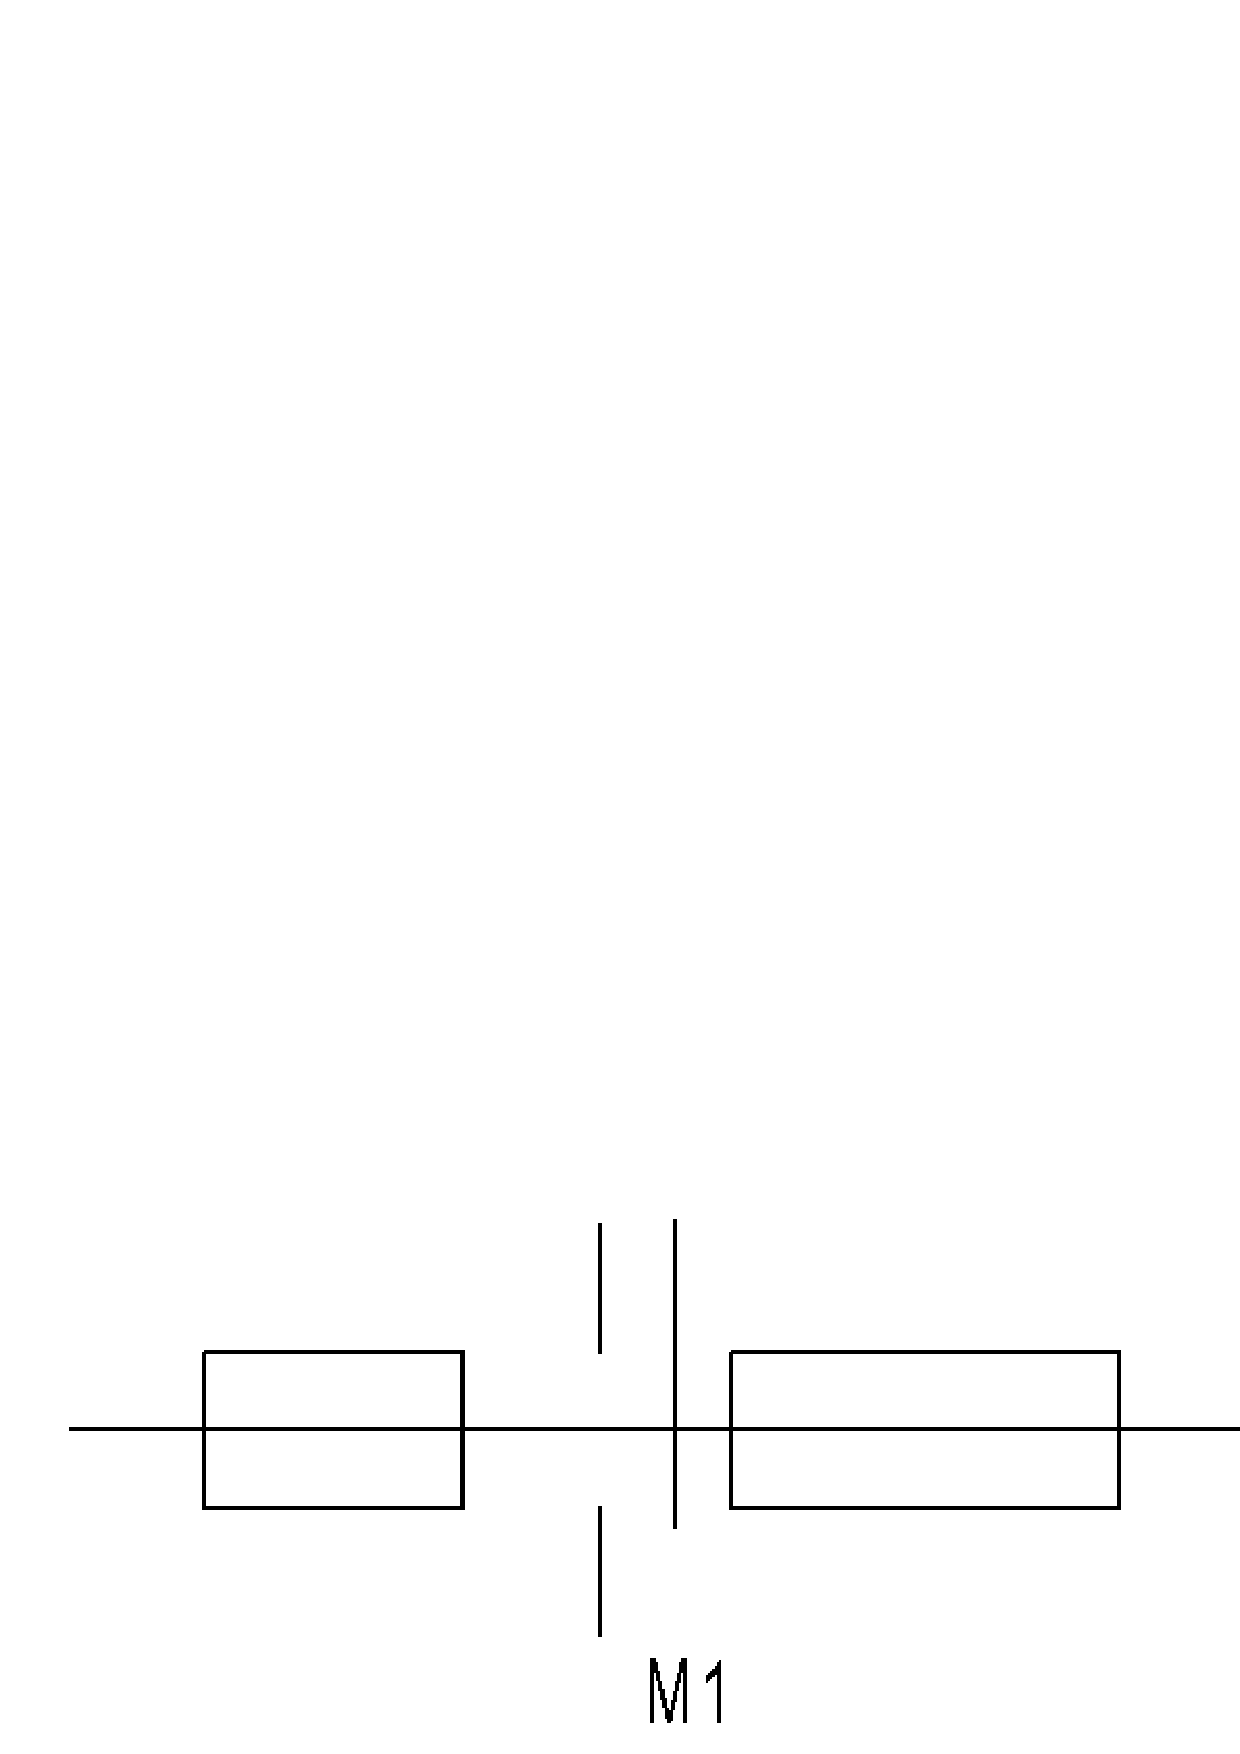
\includegraphics[width=0.6\linewidth]{2.jpg}
   	%\end{center}
   \item 计算过程
   
   	\item MATLAB代码如下
   	\begin{lstlisting}[language=MATLAB]
   %光纤光栅温度与波长的关系
   clear;clc;
   data = xlsread('C:\Users\shenda\Desktop\实验.xlsx','sheet2','A3:B10');
   lambda = data(:,1);
   T = data(:,2);
   scatter(lambda,T,'m*');
   p = polyfit(lambda,T,1);
   lambda1 = 1540:0.01:1541;
   TT = polyval(p,lambda1);
   hold on
   plot(lambda1,TT,'b','linewidth',2);
   xlabel('波长\lambda(nm)');
   ylabel('温度T(℃)');
   title('光纤光栅温度与波长的关系');
   text(1540.532,61,['\leftarrow 斜率k=',num2str(round(p(1)))],'FontSize',12);
   set(gca,'FontSize',12,'Fontname','New Times Roman');
   set(gcf, 'PaperPositionMode', 'manual');
   set(gcf, 'PaperUnits', 'points');
   set(gcf, 'PaperPosition', [0 0 1000 800]);
   print -djpeg -r600 光纤光栅温度与波长的关系
   	
   	\end{lstlisting}
   \end{clause}

 
 \subsection{做实验和处理数据过程中的问题}
 \subsection{做完实验的感悟}

\section{用m线法测量有机聚合物平面光波导的厚度和折射率}
	\subsection{实验数据处理}
	\begin{clause}
		\item 实验室测得的扫描图像如下(原始数据导出到.txt文件)
		\begin{center}
			\includegraphics[width=0.6\linewidth]{311.jpg}
		\end{center}
	\item 峰值求解图像如下
	\begin{center}
		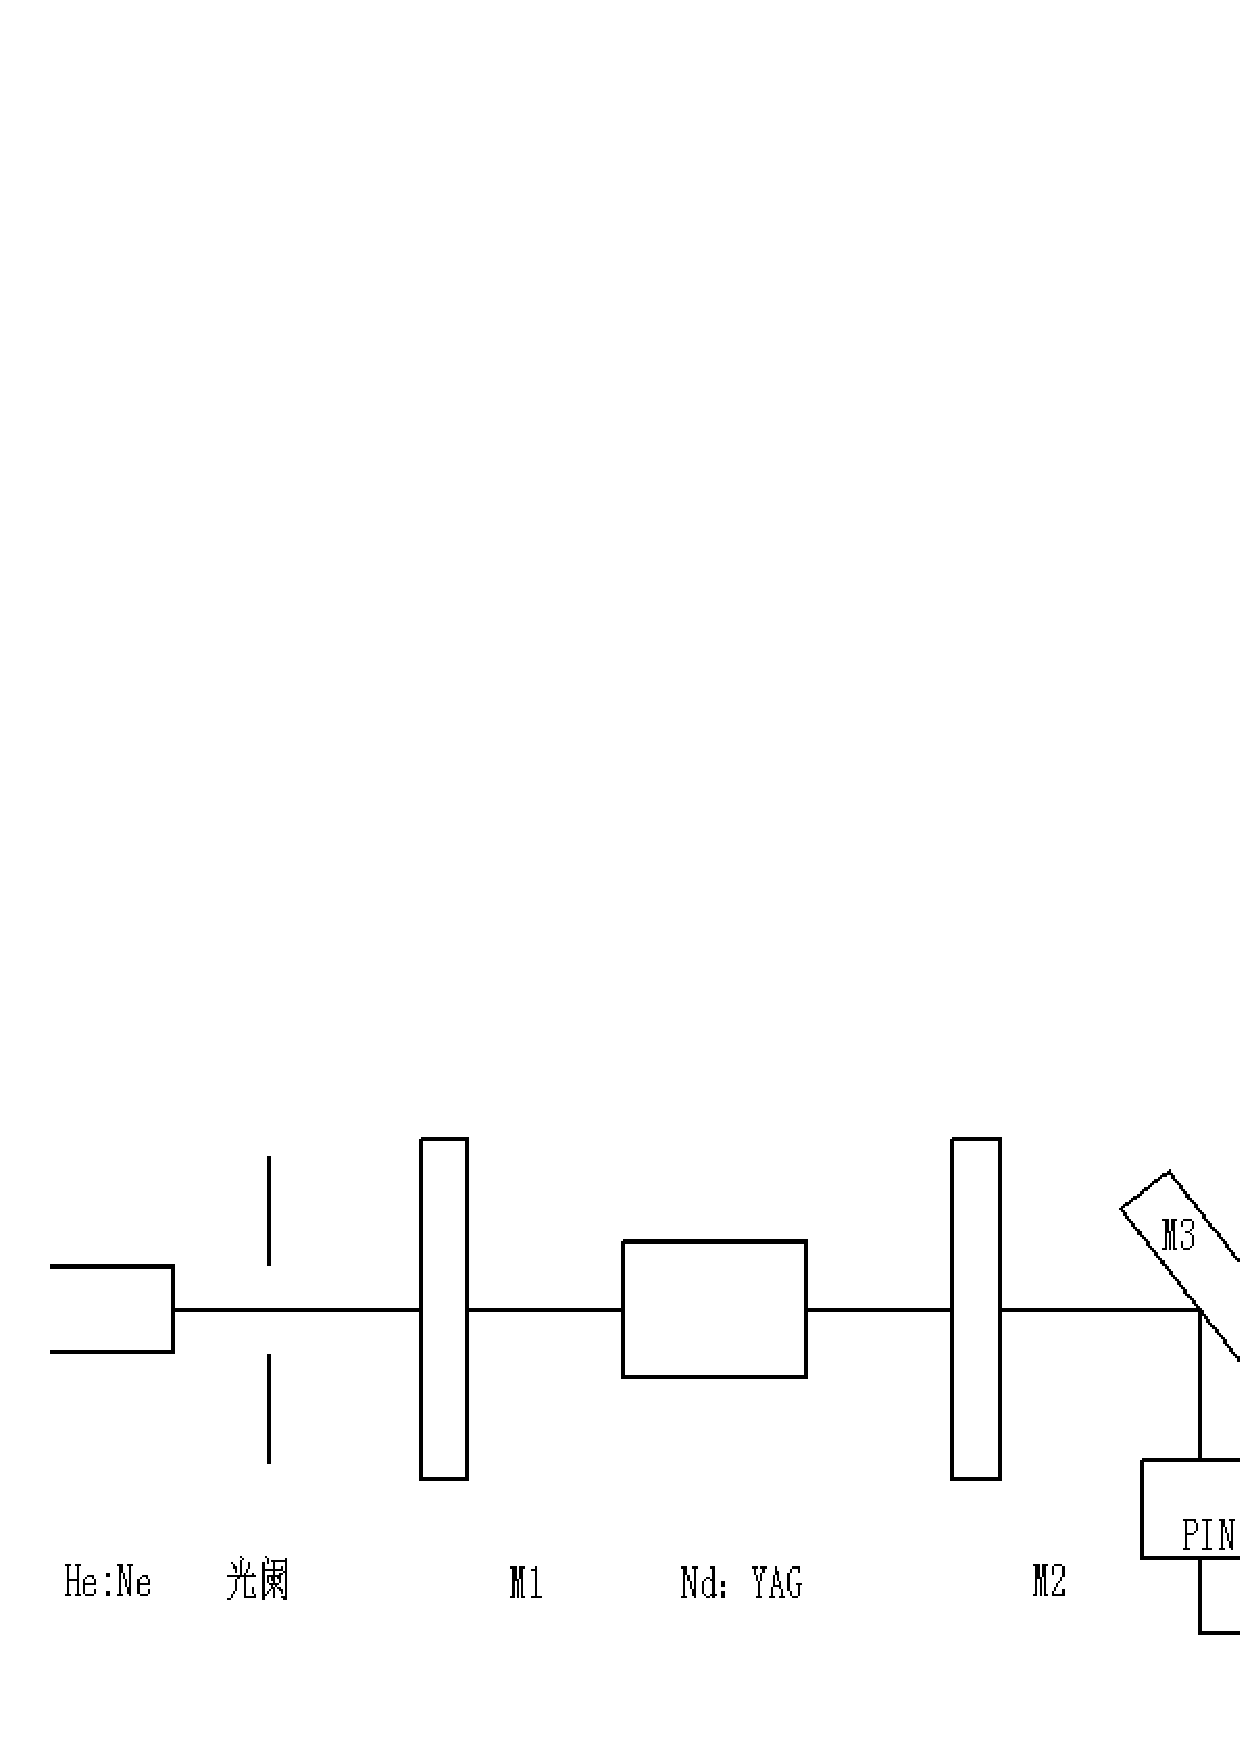
\includegraphics[width=0.6\linewidth]{3.jpg}
	\end{center}
	使用MATLAB中的findpeaks函数找到在0阶和1阶波导下的数据点,如上图所示,也就是处于波谷的两个点,在0阶波导下$(\theta,V)$为(2.9287,4.148),在1阶波导下为(4.6156,2.913)。
	\begin{center}
		\includegraphics[width=0.6\linewidth]{32.png}
	\end{center}
	根据上图所示的角度换算图
	$$n_{p}=\frac{\sin \theta}{\sin \theta\textquotesingle}$$
	$$\alpha+\theta\textquotesingle=60^{\circ}$$
	其中,$n_{p}$是三棱镜的折射率。根据以上两式,即可求得棱镜的耦合角$\alpha$
	$$\alpha=60^{\circ}-\arcsin\frac{\sin\theta}{n_{p}}$$
	将求出的$\theta_{1}=2.9287^{\circ}$和$\theta_{2}=4.6156$代入,求得$\alpha_{1}=59.9708^{\circ}$和$\alpha_{2}=59.9504^{\circ}$,即$\alpha_{m}=[\alpha_{1},\alpha_{2}]$。\\
	接下来就是求解光波的传导系数$\beta_{m}$求解如下式
	$$\beta_{m}=k_{0}n_{eff}$$
	$$k_{0}=\frac{2\pi}{\lambda}$$
	$$n_{eff}=n_{p}\sin\alpha_{m}$$
	其中,$\beta_{m}$是m阶波导的传播常数,$k_{0}$是真空中的波矢,$n_{eff}$是有效折射率。实验所用的光的波长$\lambda$约为650nm,实验所用的三棱镜的折射率$n_{p}$取缺省值1.750,计算得到$\beta_{m}=[1.464560535603606\times10^{7},1.464312266887283\times10^{7}]$
	接下来就是根据超越方程求解有机聚合物平面光波导的厚度和折射率,根据
	$$\kappa_{0}h=\arctan\frac{p_{0}}{\kappa_{0}}+\arctan\frac{q_{0}}{\kappa_{0}}$$
	$$\kappa_{1}h=\pi+\arctan\frac{p_{1}}{\kappa_{1}}+\arctan\frac{q_{1}}{\kappa_{1}}$$
	其中,h为薄膜厚度,$\kappa$,p,q可以由下式求得
	$$\kappa=\sqrt{k_{0}^{2}\epsilon_{1}-\beta_{m}^{2}}$$
	$$p=\sqrt{\beta_{m}^{2}-k_{0}^{2}\epsilon_{2}}$$
	$$q=\sqrt{\beta_{m}^{2}-k^{2}_{0}\epsilon_{3}}$$
	$$\epsilon=(n_{r}+in_{i})^{2}$$
	其中,$n_{r},n_{i}$分别代表折射率的实部和虚部,$\epsilon_{1},\epsilon_{2},\epsilon_{3}$分别为波导薄膜、衬底、金属覆盖层的介电常数。求得$\kappa,p,q$之后代入超越方程,使用MATLAB求得有机聚合物平面光波导的厚度为20.1486$\mu m$,折射率为1.5152。
		\item 求解超越方程可视化如下\\
		因为两个超越方程都是两个因变量,所以可以画出其图形就是两个曲面,之后两个曲面与z=0平面这三个面相交的点也就是我们所求的点。
		\begin{center}
%			\includegraphics[width=0.6\linewidth]{31.jpg}
		\end{center}
	
		\item MATLAB代码如下
		\begin{lstlisting}[language=MATLAB]
		%Experiment of Light Information Science&Technology
		%measure thin and reflection
		clear;clc;
		data_PI=xlsread('C:\Users\shenda\Desktop\实验.xlsx','sheet3','A3:B8851');
		%公式:角度(theta)=步数*(360 / 传动比(180) / 电机每圈步数(200) / 电机细分数(16))
		data_PI(1,:) = [];
		theta = data_PI(:,1)*(360/180/200/16);
		voltage = data_PI(:,2);
		plot(theta,voltage,'linewidth',2);hold on;
		xlabel('入射角\theta(°)');
		ylabel('光强信号电压U(V)');
		title('U-\theta扫描曲线');
		set(gca,'FontSize',10,'Fontname','Yahei Consolas Hybrid');
		box off
		%寻找峰值
		[peaks,locs] = findpeaks(-voltage,'minpeakheight',-5,'minpeakdistance',1);
		j=1;
		for i=1:1:size(locs)-1
			if(abs(locs(j+1)-locs(j))<1000)
				if(peaks(j+1)<peaks(j))
					peaks(j+1)=[];
					locs(j+1)=[];
				else
					peaks(j)=[];
					locs(j)=[];
				end
			else
				j=j+1;
			end        
		end
		%在图上标出峰值
		plot(theta(locs),voltage(locs),'*r');
		MarkLocationTheta = [theta(locs(1))+0.1 theta(locs(2))+0.1];
		MarkLocationVoltage = [voltage(locs(1)) voltage(locs(2))];
		str = {['(',num2str(theta(locs(1))),',',num2str(voltage(locs(1))),')',],['(',num2str(theta(locs(2))),',',num2str(voltage(locs(2))),')']};
		text(MarkLocationTheta,MarkLocationVoltage,str);
		box off
		print -djpeg -r600 m线法测量实验的U-theta的0阶和1阶模的曲线
		%得到耦合状态下的theta和voltage(0阶和1阶模式)
		theta_peak = theta(locs);
		theta_peakArc = theta(locs)*pi/180;
		voltage_peak = voltage(locs);
		%根据公式计算,np=1.750是三棱镜折射率
		np = 1.750;
		alpha = 60 - asin(sin(theta_peakArc)/np);
		%betam为m阶波导的传播常数,k0是真空中的波矢k0=1/lambda;
		lambda = 650*(10^(-9));%波长是650nm                                                                                                                                                                                                                                                                                                                                                                                                                                                                                                                                                                                                                                                                                                                                                                                                                                                                                                                                                                                                       
		k0 = 2*pi/lambda;%真空中的波矢
		alphaArc = alpha*pi/180;
		betam = k0*np*sin(alphaArc); 
		
		syms epsilon1 h;
		epsilon2 = 1.75^2;%三棱镜
		epsilon3 = -17.0373;%epsilon3 = (real((0.14+4.13*i)^2)),%金属略去虚部
		
		k0 = k0*[1;1];
		kapa = (k0.^2*epsilon1-betam.^2).^(1/2);
		p = (betam.^2-k0.^2*epsilon2).^(1/2);
		q = (betam.^2-k0.^2*epsilon3).^(1/2);
		x1 = kapa(1)*h;
		x2 = kapa(2)*h;
		y1 = atan(p(1)/kapa(1))+atan(q(1)/kapa(1));
		y2 = 3.14+atan(p(2)/kapa(2))+atan(q(2)/kapa(2));
		e1 = y1-x1;
		e2 = y2-x2;
		%e1,e2作图与z=0的交点
		figure(2)
		strx = (['z=\kappa_{m}h-m\pi+tan^{-1}({p_{m}}/{\kappa_{m}})+tan^{-1}({q_{m}}/{\kappa_{m}})=0 m=0,1']);
		suptitle(strx)
		set(gca,'FontSize',10,'Fontname','New Times Roman');
		subplot(2,2,1)
		ezmesh(e1);
		hold on 
		ezmesh('0')
		hold on
		ezmesh(e2);
		title('正常视角');
		zlabel('z');
		
		subplot(2,2,2);
		ezmesh(e1);
		hold on 
		ezmesh('0')
		hold on
		ezmesh(e2);
		title('主视图');
		view(0,0)
		zlabel('z');
		
		subplot(2,2,3);
		ezmesh(e1);
		hold on 
		ezmesh('0')
		hold on
		ezmesh(e2);
		title('左视图');
		view(90,0)
		zlabel('z');
		
		subplot(2,2,4);
		ezmesh(e1);
		hold on 
		ezmesh('0')
		hold on
		ezmesh(e2);
		title('俯视图');
		view(0,90)
		set(gcf, 'PaperPositionMode', 'manual');
		set(gcf, 'PaperUnits', 'points');
		set(gcf, 'PaperPosition', [0 0 1200 1080]);
		print -djpeg -r600 方程求解可视化
		%求解超越方程
		[epsilon1,h] = solve(e1,e2);
		t=double([real(epsilon1),real(h)]);
		disp('epsilon1=')
		disp(t(1));
		disp('折射率n=');
		disp(sqrt(t(1)));
		disp('波导层的厚度h(um)=');
		disp(num2str(t(2)*10^(6)));
		
		\end{lstlisting}
	\end{clause}
   \subsection{做实验和处理数据过程中的问题}
   	~\\
   ~\\
   ~\\
   ~\\
   ~\\
   ~\\
   ~\\
   ~\\
   ~\\
   ~\\
   ~\\
   ~\\
   ~\\
   ~\\
   ~\\
  \subsection{做完实验的感悟}
~\\
~\\
~\\
~\\
~\\
~\\
~\\
~\\
~\\
~\\
~\\
~\\
~\\
~\\
~\\
\section{光纤杨氏实验}
  \subsection{实验数据处理}
  \begin{clause}
  	\item 实验的原始数据如下
  	\begin{center}
  		\begin{tabular}{|c|c|}
  			\multicolumn{2}{c}{表4.1 光纤杨氏实验数据}\\
  			\hline
  			$D_{1}$(cm)&12\\\hline
  			$D_{2}$(cm)&11\\\hline
  			$\lambda$(nm)&630\\\hline
  			$x_{1i}$(共测三次,mm)&[24.71,35.08,46.72]\\\hline
  			$x_{2i}$(共测三次,mm)&[46.46,34.90,23.95]\\\hline
  		\end{tabular}
  	\end{center}
  其中,D是卡尺和显微镜之间的距离,$\lambda$是使用的光的波长,$x$是每过十个条纹在卡尺上的读数,根据式子
  $$\Delta D=|D_{1}-D_{2}|$$
  $$\Delta x_{ij}=\Delta x{i(j+1)}-\Delta x_{ij)},i,j=1,2$$
  $$\Delta x_{i}=\frac{\sum_{i=1}^{n}\Delta x_{i}}{n}$$
  $$\Delta x=|\Delta x_{1}-\Delta x_{2}|$$
  $$d=\frac{\lambda \Delta D}{\Delta x}$$
  将数据输入Excel,使用Excel的内置函数即可求得
  \begin{center}
  	\begin{tabular}{|c|c|}
  		\multicolumn{2}{c}{表4.2 处理后的实验数据}\\
  		\hline
  		$\Delta x_{1i}$(mm)&[10.37,11.64]\\\hline
  		$\Delta x_{2i}$(mm)&[11.64,10.95]\\\hline
  		$\Delta x_{1}$(mm)&11.005\\\hline
  		$\Delta x_{2}$(mm)&11.255\\\hline
  		$\Delta x$(mm)&0.25\\\hline
  		d($\mu$m)&25.2\\\hline
  	\end{tabular}
  \end{center}
  \end{clause}
其中,$\Delta x$是杨氏条纹之间的间距,d是双孔之间的距离,求得结果双孔之间的距离d=25.2$\mu $m。
     
  \subsection{做实验和处理数据中的问题}
    	~\\
    ~\\
    ~\\
    ~\\
    ~\\
    ~\\
    ~\\
    ~\\
    ~\\
    ~\\
    ~\\
    ~\\
    ~\\
    ~\\
    ~\\
  \subsection{做完实验的感悟}
  	~\\
  ~\\
  ~\\
  ~\\
  ~\\
  ~\\
  ~\\
  ~\\
  ~\\
  ~\\
  ~\\
  ~\\
  ~\\
  ~\\
  ~\\
  \subsection{思考题}
  \begin{clause}
  	\item 阶跃型光纤的纤芯折射率$n_{1}=1.52$,包层的折射率$n_{2}=1.50$,纤芯的直径2a=50$\mu$m,用$\lambda=0.8\mu$m的光作为光源。
  	\begin{itemize}
  		\item[a.] 求其数值孔径NA和最大孔径角$\theta_{m}$;
  		\item[b.] 求光纤波导的归一化频率参量、多模的个数;
  		\item[c.] 当光纤的直径是多少的时候,才能获得单模传输。
  	\end{itemize}
  \item 若采用三根以上的光纤进行多光束干涉实验,其干涉场具有什么特点,有些什么应用?
  	~\\
  ~\\
  ~\\
  ~\\
  ~\\
  ~\\
  ~\\
  ~\\
  ~\\
  ~\\
  ~\\
  ~\\
  ~\\
  ~\\
  ~\\
  \end{clause}
  
\section{基于光纤sagnac干涉原理的全光纤声学传感系统}
  \subsection{实验数据处理}
    \begin{clause}
    	\item 单一频率信号\\
    	使用实验室的单一频率信号发生软件,得到一个单一的正弦波信号的时域和频域图如下
    	\begin{center}
    		\includegraphics[width=0.6\linewidth]{5.1.jpg}
    	\end{center}
       	\item 多频率复杂信号处理\\
       	之后在实验室录了一首歌,求得其时域、频域和短时能量图如下\\
       	\begin{center}
       		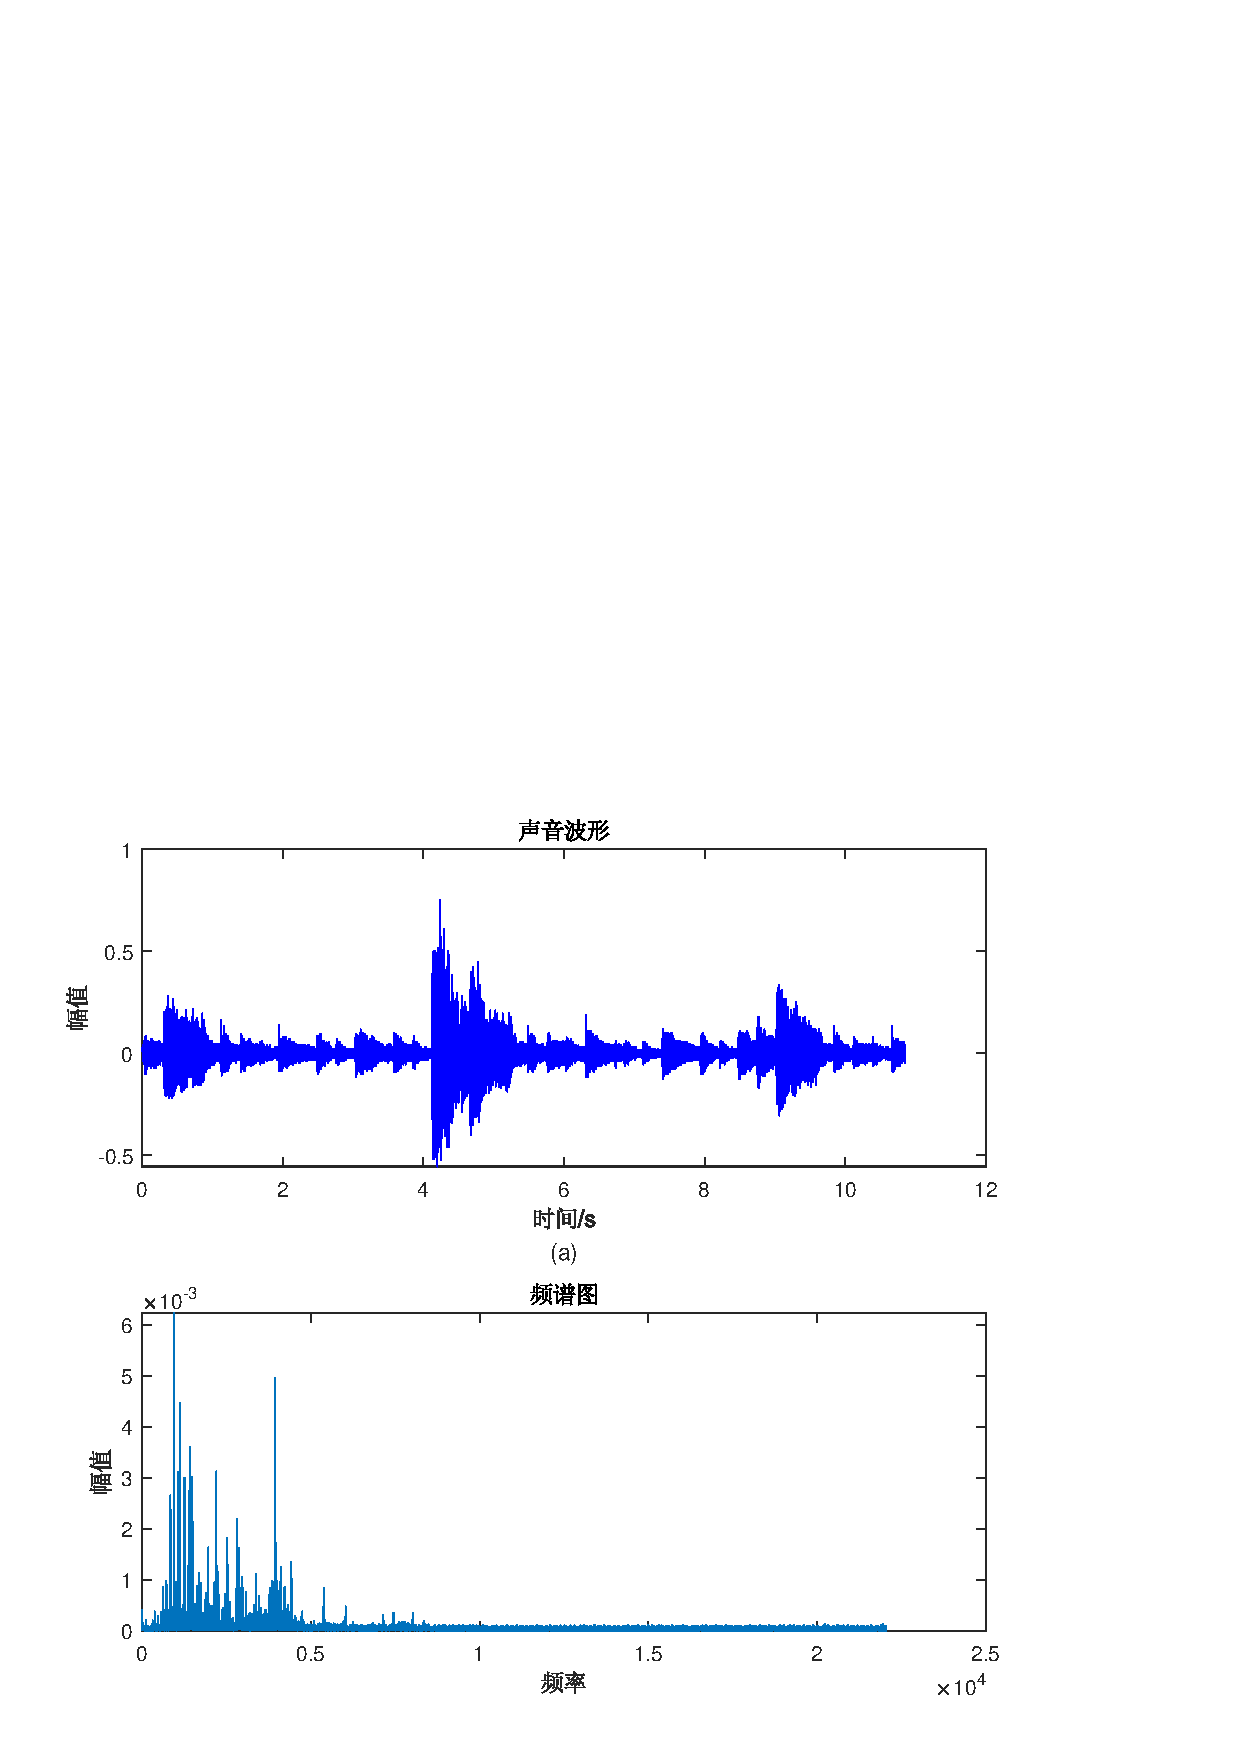
\includegraphics[width=0.6\linewidth]{5.2.jpg}
       		\includegraphics[width=0.6\linewidth]{5.21.png}
       	\end{center}
       通过设计MATLAB的fdatool工具箱来设置滤波器,设置一个低通滤波器,滤波方法是IIR,切比雪夫II型,通频5kHz,截止频率为6kHz,滤波器的参数设置和频率响应如下:
       \begin{center}
       	\includegraphics[width=0.6\linewidth]{5.31.png}
       	\includegraphics[width=0.6\linewidth]{5.3.png}
       \end{center}
   		在MATLAB的Simulink中,设计如下的模型来仿真滤波
   		\begin{center}
   			\includegraphics[width=0.6\linewidth]{5.4.png}
   		\end{center}
   	没有滤波和滤波后频域如下
   	\begin{center}
   			\centering
   			\includegraphics[width=0.6\linewidth]{5.41.png}
   		\end{center}
   	\begin{center}
   		\includegraphics[width=0.6\linewidth]{5.5.png}
   	\end{center}
   前后的时域信号如下
   \begin{center}
   	\includegraphics[width=0.6\linewidth]{5.52.jpg}
   	\includegraphics[width=0.6\linewidth]{5.51.jpg}
   \end{center}
	可以看到,经过滤波器后,高频成分大幅减少,信号强度也有所削减。
    之后又设计了一个带通滤波器,也是加入上述的Simulink模块进行仿真,其滤波后的频域和时域图如下
     \begin{center}
    	\includegraphics[width=0.6\linewidth]{5.61.jpg}
    	\includegraphics[width=0.6\linewidth]{5.62.jpg}
    \end{center}
	可以看到,在前面一段有低频信号被滤除,保留的是1~5kHz之间的频率部分,信号的强度相对于低通滤波器没有很明显的减少,这就说明1~5kHz这部分的信号强度在这首歌曲里面占的是主导地位
    	\item MATLAB处理代码
    	
    	\begin{lstlisting}[language=MATLAB]
    	clear;clc;
    	[x,Fs] = audioread('C:\Users\沈达\Desktop\光信息实验\wang1.wav');
    	wlen = 200;inc = 80;
    	win = hanning(wlen);
    	N = length(x);
    	X = enframe(x,win,inc)';
    	fn = size(X,2);
    	time = (0:N-1)/Fs;
    	for i=1:fn
    	u = X(:,i);
    	u2 = u.*u;
    	%     En(i) = sum(u2);
    	end
    	figure(1)
    	subplot 211
    	plot(time,x,'b');
    	title('声音波形');
    	ylabel('幅值');xlabel(['时间/s',10,'(a)']);
    	Y = fft(x);
    	f = Fs*(0:(N/2))/N;
    	P2 = abs(Y/N);
    	P1 = P2(1:N/2+1);
    	P1(2:end-1) = 2*P1(2:end-1);
    	subplot 212
    	plot(f,P1);
    	title('频谱图')
    	xlabel('频率');ylabel('幅值');
    	print -djpeg -r600 多频率的声音信号的频谱图(实验室产生的单一频率声音)
    	\end{lstlisting}
    	
    
    	
    \end{clause}
  \subsection{做实验和处理数据中的问题}
  	~\\
  ~\\
  ~\\
  ~\\
  ~\\
  ~\\
  ~\\
  ~\\
  ~\\
  ~\\
  ~\\
  ~\\
  ~\\
  ~\\
  ~\\
  \subsection{做完实验的感悟}
  	~\\
  ~\\
  ~\\
  ~\\
  ~\\
  ~\\
  ~\\
  ~\\
  ~\\
  ~\\
  ~\\
  ~\\
  ~\\
  ~\\
  ~\\
   \subsection{思考题}
   \begin{clause}
   	\item 实验中添加的偏振控制器,它的作用是什么?(提示:从o光和e光的定义出发)
   	\item 实验中的噪声来源有哪些?
   	\item 上面提到理想的萨格那克环使用5:5耦合器情况下为全反射,那么当使用的耦合器不是5:5的情况下还会全反射吗(不考虑非线性效应)?
   		~\\
   	~\\
   	~\\
   	~\\
   	~\\
   	~\\
   	~\\
   	~\\
   	~\\
   	~\\
   	~\\
   	~\\
   	~\\
   	~\\
   	~\\
   \end{clause}
\subsection{参考文献}
\begin{clause}
	
	\item 明海,张国平,谢建平;“光电子技术",中国科学技术大学出版社,合肥,1998
\end{clause}
\end{document}
